	\section{Experimental Evaluation}
	
	We implemented our code in Python 3.8.
	Gurobi 9.52 was used for solving the MILP problems. We conducted our evaluation on an AMD Threadripper 7970X ($32$ cores$@4.0$GHz) with 256 GB of main memory and 2 NVIDIA RTX 4090. 
	
	We consider two DNNs: one for MNIST, namely a pre-trained $5\times 100$ (available at \url{https://github.com/eth-sri/eran}), a 5 fully connected layers DNN, with 100 neurons each,	trained with diff AI \cite{deeppoly}. 
	Although it is relatively small, it is also of good quality with $97\%$ accuracy on classification, but it is not easy to certify for global robustness (the size of a network can be deceptive to know whether they are easy or hard to verify \cite{ATVA25}).  
	The second one is a 2 fully connected layers, 50 neurons each, learnt as a surrogate model, with 10 reduced input and 26 reduced output, that predictS the plastic strain in 3000 points of a mesh over a pipe given the deformation of each of this 3000 points (through a PCA order reduction \cite{Paco} encoding all 3000 points with 10 dimensions in input and 26 dimensions in output), from \cite{aiware}.
	
	MNIST is a classification benchmark, we thus compute the different $\beta^{\varepsilon}_{i,j}$ bounds, for an $L_1$-deformation $\varepsilon = \leq .5$. 
	The pipe considers a conjunction of 
	$L_1 \leq 3.9$ and $L_\infty \leq .02$ perturbations, physically pertinent dimensions, and maximizes the sum of the difference in output of 10 selected points in the mesh between input and its deformation.

For each benchmark, we report three values: the bound obtained (lower value is better), the solution obtained (distance to the bound depicts how close the model has converged), and worst-case (higher is better), that is the value reached when considering the solution as input to the DNN. For a fully accurate model ("2v" or classical and all variables binary), the worst-case will equal the solution, otherwise, it will be smaller due to abstraction.

\subsection{Classical vs our "2v" model vs ITNE}


\begin{table}[b!]
	\centering
	\begin{tabular}{||l|c|c|c||}\hline\hline
		model &        Bound $\downarrow$ &  Sol. &      Worst-Case $\uparrow$ \\\hline \hline
	Classical, $50 \times 2$ &    $.320$ &  $.320$ & $.017$ 
    \\\hline
	ITNE, $50 \times 2$ &    $.042$ &  $.037$ & $.022$
	\\ \hline
    2v model, $50 \times 2$ &    {\bf .040} &  $.037$ &  $.018$ 
    \\\hline \hline
    Classical, $100 \times 2$ &  .186  &  $.022$ & $.022$ 
    \\\hline
	ITNE, $100 \times 2$ &    $.045$ &  $.023$ & .023
    \\\hline
	2v model, $100 \times 2$&     {\bf .042} &  $.023$ &   .023 
    \\\hline \hline
	\end{tabular}
	\caption{Comparison of the classical encoding, ITNE and our "2v" model on the pipe system with a fixed timeout of 1000s, with either $50 \times 2$, 
    or the full $100 \times 2$ binary variables.}
    \label{table.classical}
\end{table}

We start by evaluating how accurate the 2v model is vs the classical encoding vs the interleaving twin-network encoding (ITNE) from \cite{lipshitz}, that we reimplement in Gurobi by considering the classical encoding plus the explicit constraints $\frac{x_i-x_i' - \gamma}{2} \leq \hat{x}_i-\hat{x}_i' \leq \frac{x_i-x_i' + \gamma}{2}$, corresponding to Eq. (3) of \cite{ITNE} (and also to our (\ref{eq.lpr})). We compare when half the ReLUs are approximated with the LP relaxation, and when all the ReLUs are encoded exactly. We use the pipe models which is easier to verify, and set the time-out at 1000s for all models.


Table \ref{table.classical}, $50 \times 2$, confirms that the LP relaxation of the classical model is extremely poor, with bounds $8$ times worse than using our "2v" model, when 50 variables use LP relaxation. Adding explicitly LP relaxation constraints of Eq. (3) from \cite{ITNE} recovers most but not all the bound of the "2v" model.

Further, even using a fully accurate model with all $100 \times 2$ variables encoded as binary variables, the "2v" model produces bounds $>4$ times better than the classical model, due to the internal Branch and Bound process to compute bounds, which uses linear relaxation. Again, 
Eq. (3) from \cite{ITNE} recovers most but not all the accuracy of the "2v" model.
Overall, the "2v" model produces better bounds, even with short time-outs, despite its higher complexity.

	\subsection{Experimental results for robustness (MNIST)}
	
We then turn to the MNIST classification benchmark, and report 
in Table \ref{table.mnist} one particular bound $\beta^{.5}_{i,j}$, namely for $i=6,j=8$ as confusion between 6 and 8 happens.
	
	\begin{table}[h!]
		\centering
	\begin{tabular}{||l||c|c|c||}\hline\hline
		model &        Bound $\downarrow$ &  Sol. &      Worst-Case $\uparrow$ \\\hline \hline
		1v, $500 \times 1$ & {\bf 14.97} & $.845$ & $.009$ \\\hline 
		3v, $500 \times 3$ & $17.66$ & $.813$ & {\bf .518} \\\hline 
	    2v, $500 \times 2$ & $16.49$ & n/a & n/a \\\hline\hline	 
	\end{tabular}
	\caption{Bounds on $\beta^{.5}_{6,8}$ 
	obtained by the "1v", "3v" and "2v" models 
	on the {\bf full dimension} MNIST DNN, 
	for timeouts of $14400$s, when all 500 ($\times 1$, $\times 2$, $\times 3$) variables are binary.}
	\label{table.mnist}
\end{table}

On the full space, the best bounds $(\beta^{.5}_{i,j})_{i < j \leq 10}$ reached are too pessimistic: no image can be certified robust in real-time. One of the reason, besides that the verification question is very complicated with 1000 binary variables for the accurate model, is that working in the full $784$ dimensional space allows for very unlikely inputs, far away from what the DNN has learnt from, making the search very long and the bound very pessimistic. As an illustration of that, we display on Fig.~\ref{fig3} the worst-case as found by our models, which is very improbable to be ever encountered in the MNIST benchmark.

\begin{figure*}[t!]
	\centering
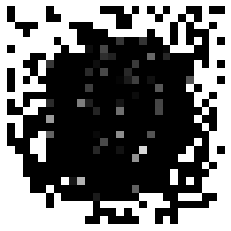
\includegraphics[scale=0.6]{image.png} \hspace{1.5cm}
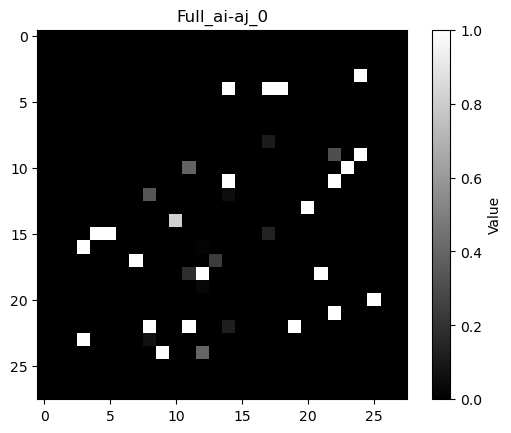
\includegraphics[scale=0.6]{perturb.png}
\caption{An improbable image for MNIST and its perturbation ($L1$-difference of $.5$ in a unique pixel at x=14, y=8 from top) with maximal $\beta^{.5}_{6,8}=0.518$, as obtained by the "3v" $500 \times 2$ model in {\bf full 784 dimension} image space.}
\label{fig3}
\end{figure*}	

\begin{figure*}[t!]
	\centering
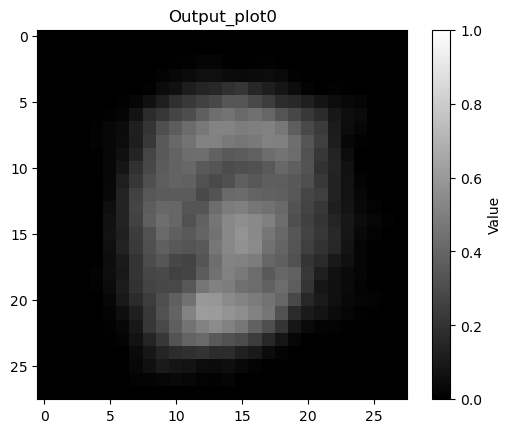
\includegraphics[scale=0.5]{redimage.png} \hspace{1.5cm}
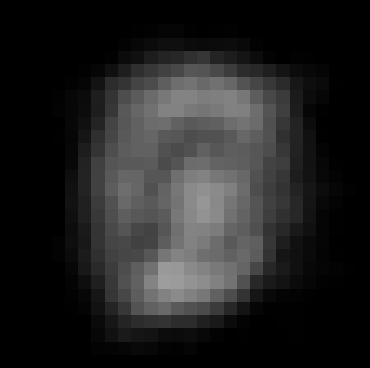
\includegraphics[scale=0.5]{redperturb.png}
\caption{An image for MNIST and its perturbation from the {\bf 20-dimension reduced space} with maximal $\beta^{.5}_{6,8}=.084$, as obtained by the "2v" $500 \times 2$ model.}
\label{fig4}
\end{figure*}	


\begin{table}[b!]
	\centering
	\begin{tabular}{||l||c|c|c||}\hline\hline
		model &        Bound$\downarrow$ &  Sol. &      Worst-Case$\uparrow$ \\\hline \hline
%1v, $400 \times 1$ & $1.414$ &  $.691$ & $.010$ \\\hline 
%3v, $400 \times 3$ & $1.186$ & $.600$ & $.003$ \\\hline 
%2v, $400 \times 2$ & $1.274$ & $.566$ & $.002$ \\\hline\hline
	 
%1v, $475 \times 1$ &  $1.408$ & $.301$ & $.008$  \\\hline 
%3v, $475 \times 3$ &  $1.153$ & $.250$ & $.006$ \\ \hline 
%2v, $475 \times 2$ &  $1.247$ & $.1957$ & $.019$ \\\hline\hline

1v, $500 \times 1$ & $1.412$ & $.161$ & .057 \\\hline 
3v, $500 \times 3$ & {\bf 1.137} & $.103$ & $.065$\\\hline 
2v, $500 \times 2$ &  $1.182$ & $.084$& {\bf .084}  \\\hline\hline
	 
	\end{tabular}
	\caption{Comparison of "1v", "3v" and "2v" models 
	to obtain bounds on $\beta^{.5}_{6,8}$ on the {\bf 20 dimension} reduced order MNIST DNN, for timeout of 14400s, where 
	all %400, 475,  or 
	500 ($\times 1$, $\times 2$, $\times 3$) neurons use binary variables.}
	\label{table.reduced}
\end{table}


\paragraph{Reduced Space}



\begin{table}[b!]
	\begin{tabular}{||l||c|c|c|c||}\hline\hline
		model &    $L_1\leq 0.5$ & $L_1\leq 1$ & $L_1\leq 1.5$ &  $L_1\leq 2$ \\\hline \hline
		1v, $500\times1$ & $80 \%$ & $32\%$ & $7\%$ & $0\%$ \\\hline
		3v, $500 \times 3$ & {\bf 86 \%} & {\bf 53\%} & {\bf 20\%} & {\bf 4\%} \\\hline
		2v, $500 \times 2$ & 84\% & 51\% & 16\% & {\bf 4\%} \\\hline \hline
	\end{tabular}
	\caption{Percentage of images certified robust in real-time 
	using the computed $(\beta^{.5}_{i,j})_{i < j \leq 10}$ 
	by the "1v", "3v" and "2v" models, for different values of $L_1$-perturbations.}
    \label{table.cert}
\end{table}


To remove improbable images and limit the space of search, 
we consider a PCA model order reduction \cite{Paco}: We reduced to 20 dimensions, because the MNIST $100 \times 5$ DNN considered, once run on images obtained from projecting to the 20 dimension space and projected back to the full dimension space displays the same accuracy of $97$\% as the DNN on the original images. This means that considering the reduced 20 dimensional space
does not incur any loss in accuracy, which is the only thing which matters. On this reduced space, bounds obtained are much more precise, and one can certify in real-time robustness of images.





We report in Table \ref{table.reduced} the same $\beta^{.5}_{6,8}$
as in Table \ref{table.mnist}, obtained with the same time-out. The bounds are directly comparable: the best $\beta^{.5}_{6,8}$ obtained using the reduced dimension is $>10$ times smaller than when using the full dimension ($1.137$ vs $14.97$). 
With these bounds, most images ($86\%$) can be certified in real-time robust for a perturbation $L_1 \leq .5$, and even $53\%$ with a perturbation $L_1 \leq 1$ twice as large, see Table \ref{table.cert}. We illustrate that improbable images are removed by displaying in Fig.~\ref{fig4} the worst-case obtained for $\beta^{.5}_{6,8}$, which indeed looks like a realistic MNIST instance.




	
	


	


\subsection{Experimental results for regression (Pipe strain)}


	\begin{figure*}[t!]
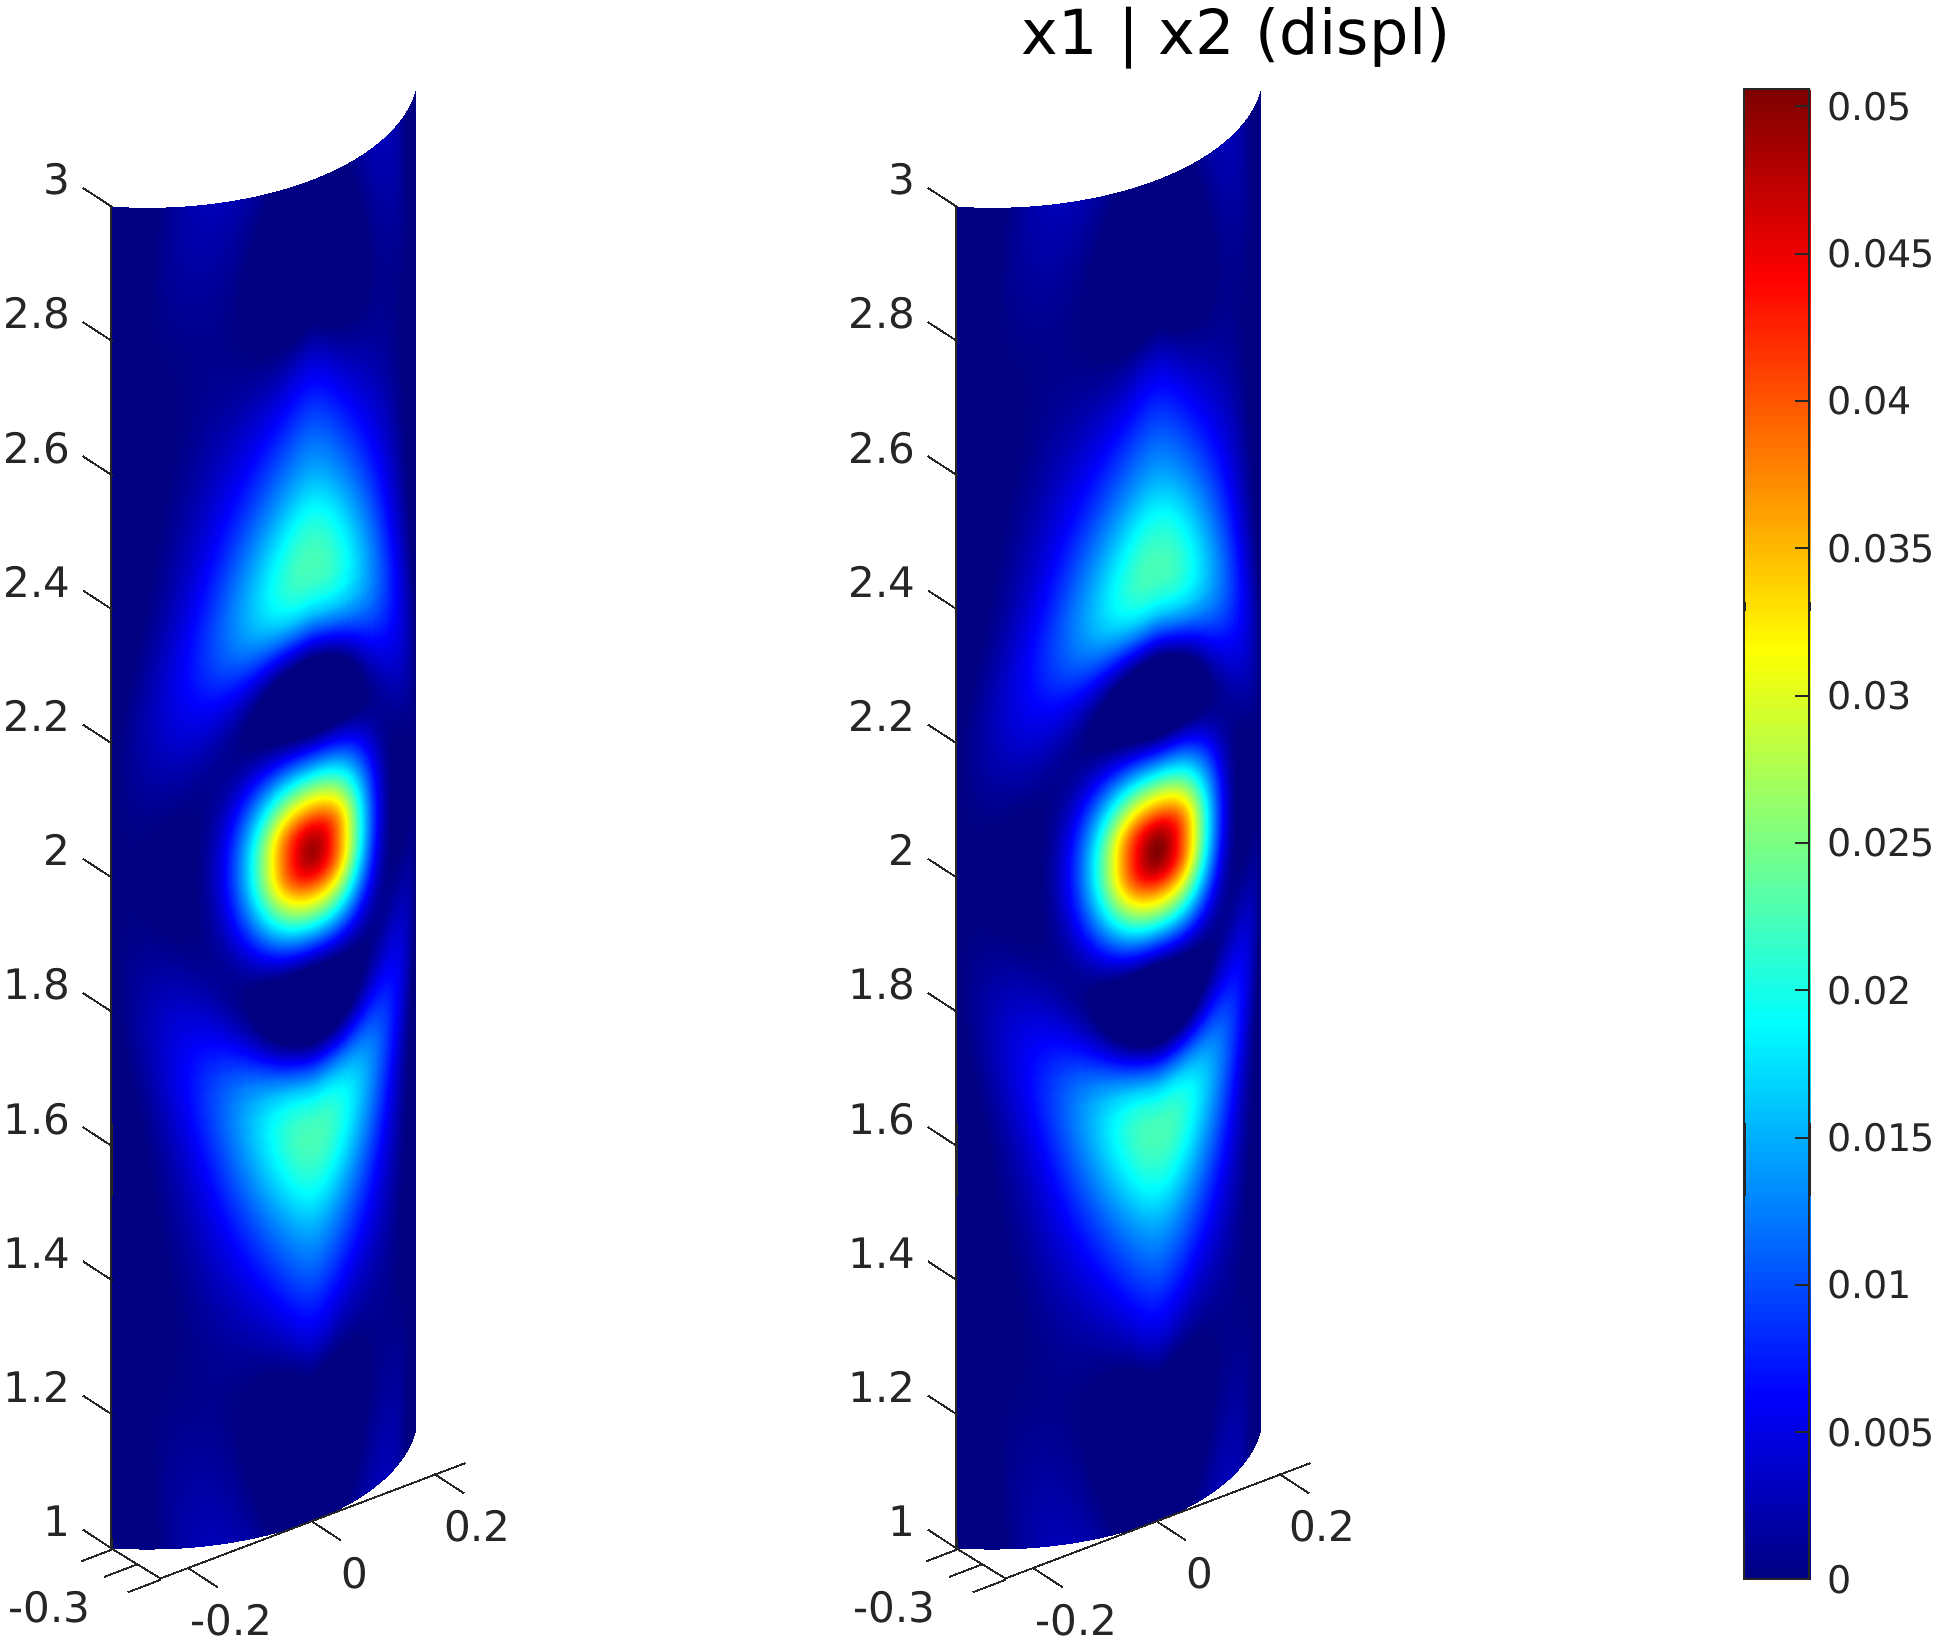
\includegraphics[scale=0.5]{deform.png} \hspace{0.8cm}
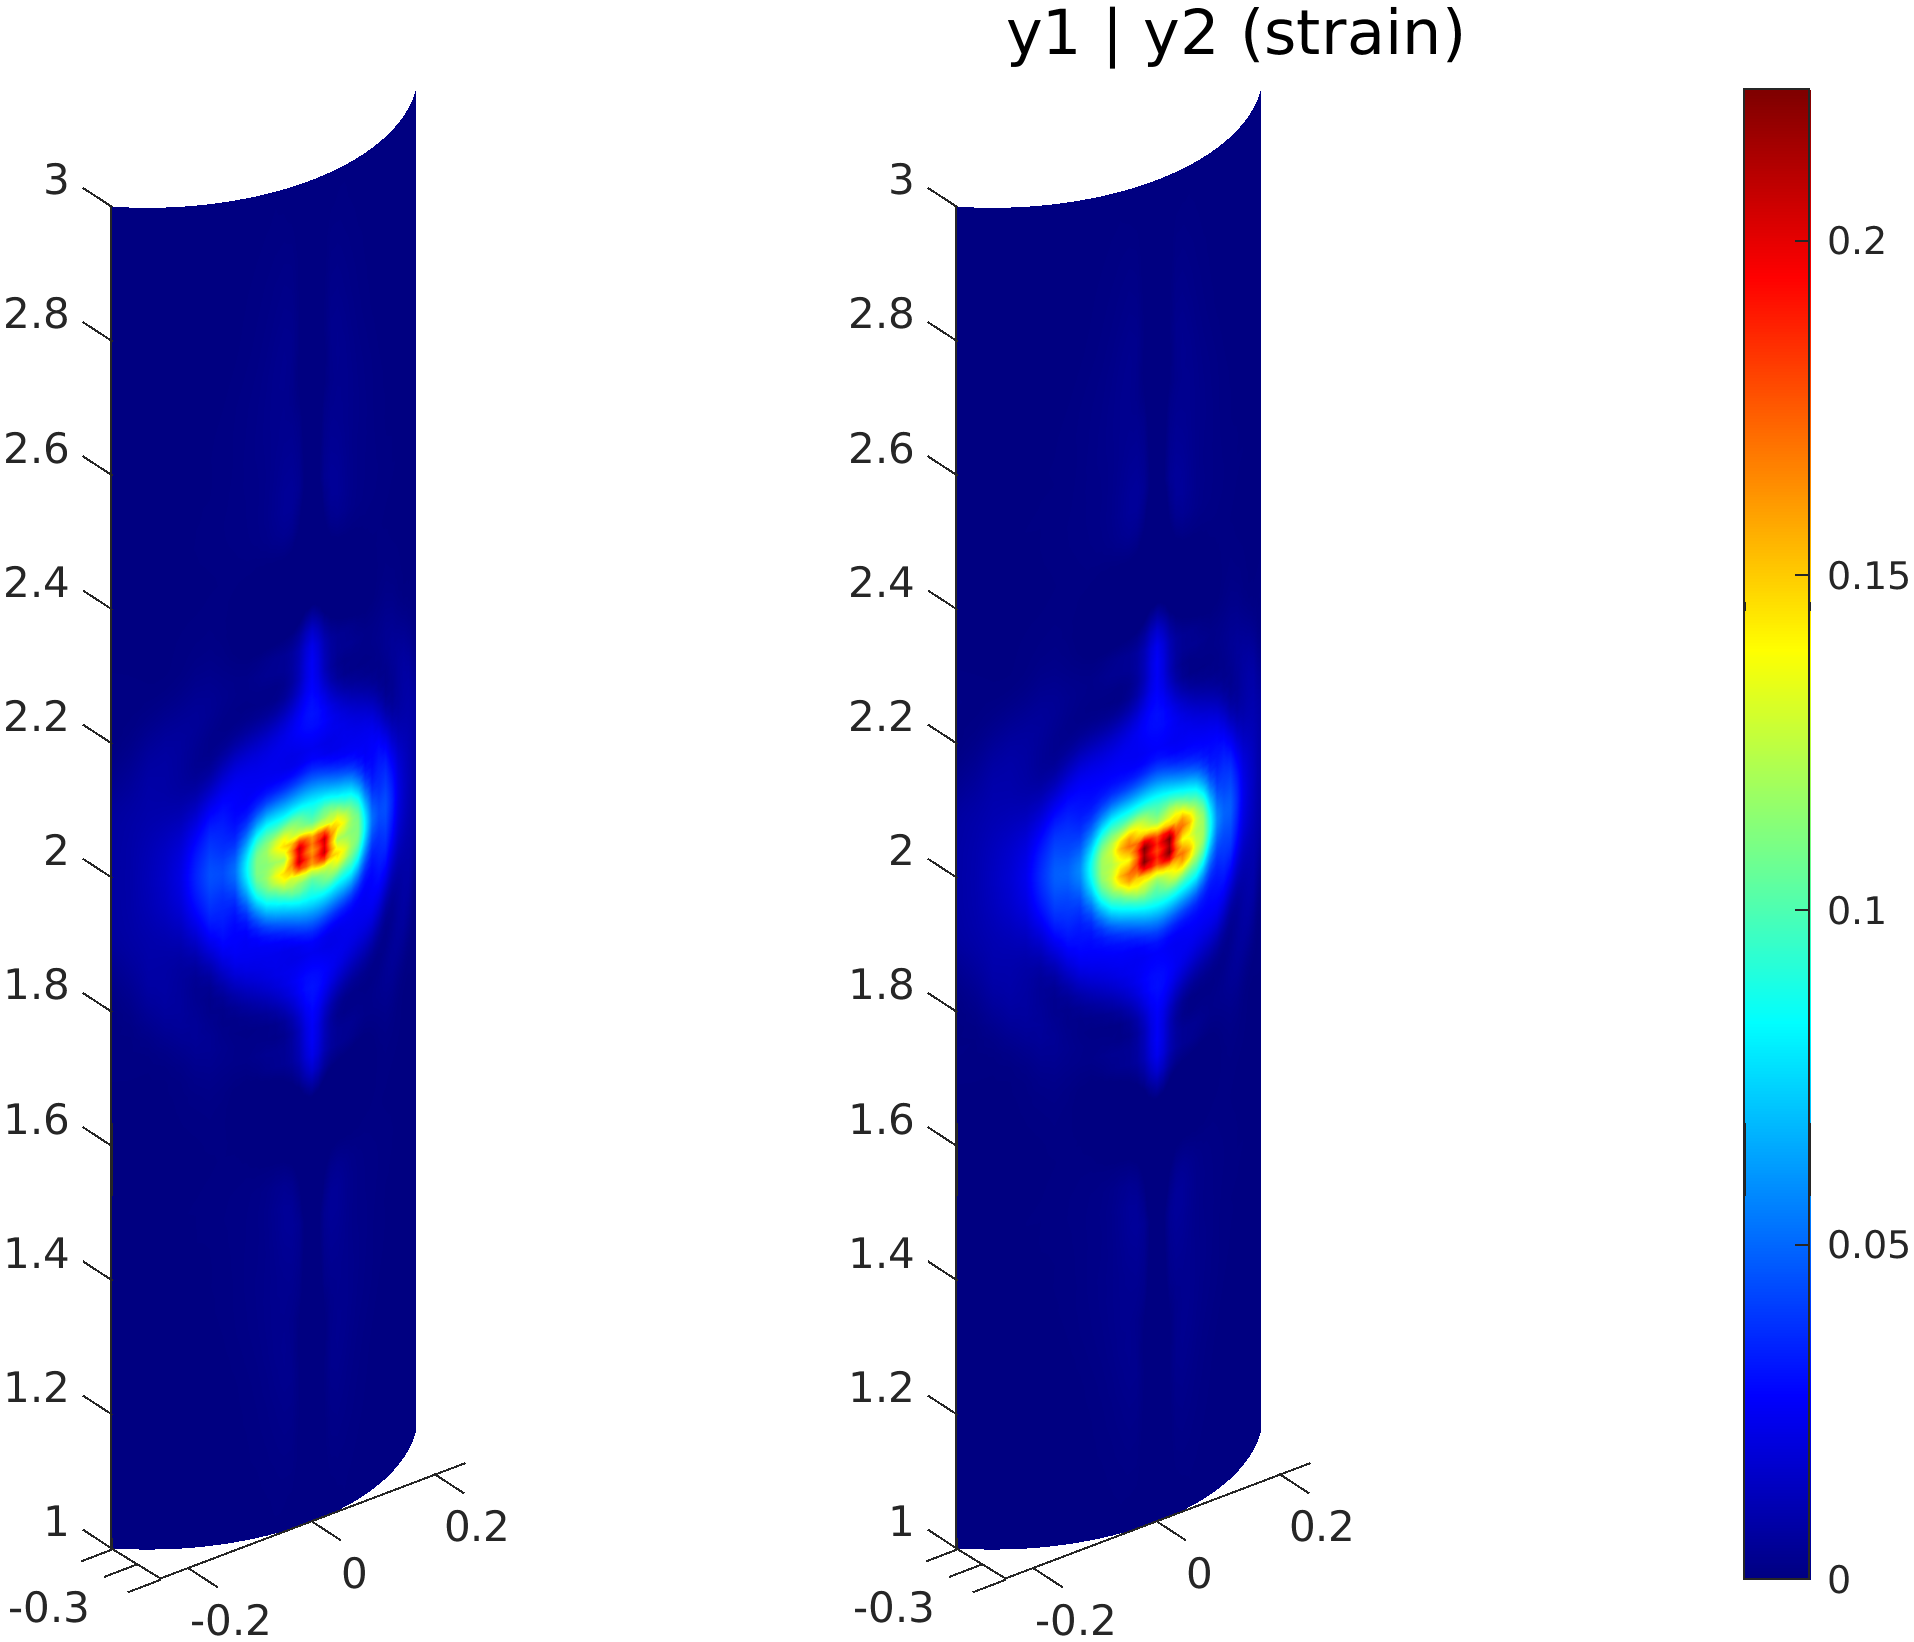
\includegraphics[scale=0.5]{strain.png}
\caption{2 slightly different deformations and their associated quite different strain as obtained by the "2v" $100 \times 2$ model.}
\label{fig5}
\end{figure*}	


	For the pipe system, we compared in Table \ref{table.pipe} the different models "1v","2v","3v" to produce bounds on the sum of the difference of strain over 10 specific points of the mesh, for a physically relevant perturbation of the deformation. The bounds we found are quite accurate, with a best bound of $.0329$ obtained by the "3v" model, slightly better than the bound $.0337$ found within the same time by the "2v" model, and better than the bound found $0.356$ by the "1v" model, although this bound has been found 70 times faster due to the simpler model. The certified lower bound is not too far, at $.245$, found by the fully accurate "2v" model when all the variables are binary. We did check that this worst-case found, displayed in Fig. \ref{fig5} and which is not too far from the actual worst case that is known to be $<.0329$, is coherent with the physical dinite element model the DNN surrogate has been learnt from, hence this is not an hallucination due to the brittleness of the learnt DNN.


	
	\vspace*{1ex}
	
	\iffalse
	\begin{table}[h!]
	\begin{tabular}{|l|l|l|l|l|}\hline
		$L_1\leq 0.83$ &        Bound $\downarrow$ &  Solution $\uparrow$ &      Real $\uparrow$ &  Time \\\hline
		1v,open 100 &     {\bf 0.035613} &  0.035613 &                       0.01288 & 10608 \\\hline
		3v,open 100 &     0.040074 &  0.028934 &                      0.021441 & 10922 \\\hline
		%3v,open 100 &     0.039824 &  0.028832 &                      0.022255 & 22153 \\\hline
		2v,open 100 &     0.046719 &  0.024364 &  {\bf 0.024436} & 10922 \\\hline
	\end{tabular}
	\caption{Comparison of 1v,2v and 3v models on the pipe system with a fixed timeout of 10.000s.}
\end{table}
\fi
	
		
	\begin{table}[h!]
	\begin{tabular}{||l||c|c|c|c||}\hline\hline
		model &        Bound$\downarrow$ &  Sol. &      Worst-Case$\uparrow$ &  Time(s) \\\hline \hline
		1v, $100 \times 1$ &     {\bf .0356} &  $.0356$ & $.0191$ &  1000 \\\hline
		3v, $100 \times 3$&     .0414 &  .0254 &  .0166 &  1000 \\\hline
		2v, $100 \times 2$&     .0418 &  .0229 &   {\bf .0229} &  1000 \\\hline \hline
		%3v, $97 \times 3$&      ?? &  ?? &  ?? & 14440 \\\hline
		3v, $100 \times 3$&      {\bf .0350} &  .0272 &  .0216 & 14440 \\\hline
		%2v, $97 \times 2$&     ?? &  ?? &   ?? & 14440 \\\hline
		2v, $100 \times 2$&     .0360 &  .0236 &    {\bf .0236} & 14440 \\\hline \hline
		3v, $100 \times 3$&     {\bf .0329} &  .0277 &  .0165 & 72000 \\\hline
		2v, $100 \times 2$&     .0337 &  .0245 &  {\bf .0245} & 72000 \\\hline\hline
	\end{tabular}
	\caption{Comparison of "1v", "3v" and "2v" models on the pipe system with timeouts of 1000s, 14440s and 72000s, where all 100 ($\times 1, \times 2,\times 3$) neurons use binary variables.}
	%L1 corresponds to $3.9$ or $4$, and results should be the sum of 10 pixels, so around 10 times higher values.}
	\label{table.pipe}
\end{table}

\newpage

\noindent {\bf Supplementary material content:} We provide in supplementary materials additional content, in particular results with reduced number of binary variables. We also provide the proof of Prop.~\ref{Prop2}, and explanations on the reduced-order dimension pipeline.